\documentclass[11pt, a4paper]{article}
\usepackage[latin1]{inputenc}
\usepackage{pgfplots}
\usepackage{pgfplotstable}
\usepackage{float}
\pgfplotsset{width=0.85\textwidth ,compat=1.9}
\usepackage[dutch]{babel}
\usepackage{csquotes}
\usepackage{amsmath}
\usepackage[toc,page]{appendix}
\usepackage{amsfonts}
\usepackage{amssymb}
\usepackage{graphicx}
\usepackage{caption}
%\usepackage[backend=biber, style=numeric, citestyle=numeric-comp, sorting = none]{biblatex}
\usepackage[backend=bibtex, style=numeric, citestyle=numeric-comp]{biblatex}
\author{Stef Tweepenninckx, r0677232}
\title{Practicum 3: Image Compositing algoritme}



%define printtitle
\makeatletter
\def\printtitle{                 
    {\large \@title}} 
\makeatother

%define printauthor
\makeatletter                       
\def\printauthor{                  
    {\large \@author}}              
\makeatother

\begin{document}
\begin{titlepage}
\newcommand{\HRule}{\rule{\linewidth}{0.5mm}} 
\center 
\textsc{\LARGE Gegevensstructuren en algoritmen}\\[1.5cm] 
\HRule \\[0.4cm]

{\huge \bfseries \printtitle}\\[0.4cm] 
\HRule \\[0.4cm]

\Large \emph{Author:}\\
 \textsc{\printauthor}\\[3cm]

{\large \textsc{18 mei 2018}}\\[3cm] 

\vfill 
\end{titlepage}

\section*{Inleiding}

\newpage
\section*{Kortste pad}
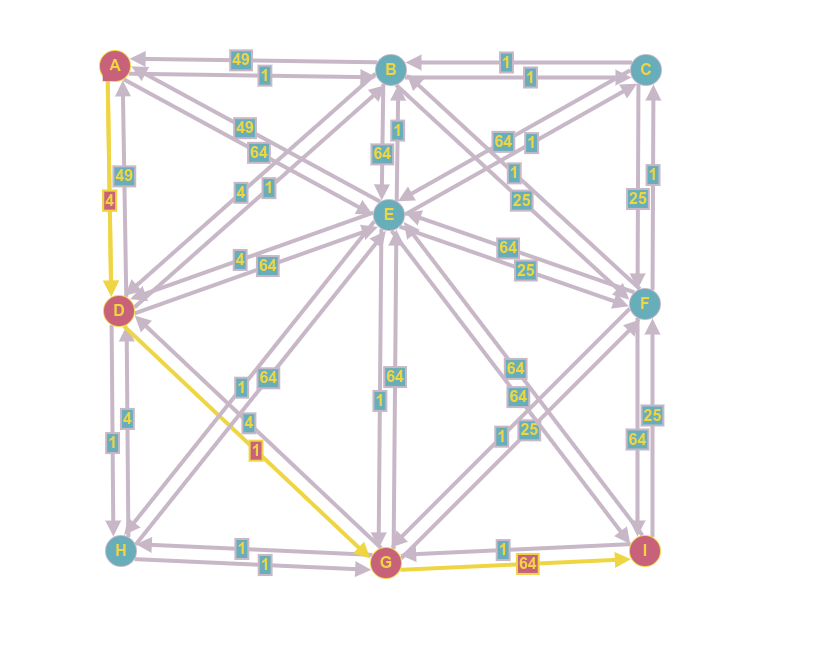
\includegraphics[width=\textwidth]{grafe}
\captionof{figure}{Grafe met aangeduid kortste pad}
\vspace*{10px}
Het resulterende kortste pad, aangeduid in het geel, is: $$A \implies D \implies G \implies I$$ met een totale kost van $49 + 4 + 1 + 64 = 118$.

\newpage
\section*{Andere afstandsfunctie}
Als we de nieuwe afstandsfunctie zouden gebruiken (gegeven in de opgave), houden we geen rekening meer met de blauwe component van een pixel. Aangezien we hierdoor minder berekeningen gaan doen, zal deze functie in de praktijk bij bijna iedere afbeelding een snellere uitvoeringstijd hebben.\\

Indien we gebruik maken van de oude afstandsfunctie, wordt eerst positie (0,1) gekozen. Daarna positie (1,0) en dan uiteindelijk eindpositie (1,1). Dijkstra heeft dus 3 stappen nodig om het einde te bereiken met de oude afstandsfunctie. Als we de nieuwe afstandsfunctie gebruiken zullen we rechtstreeks van (0,0) naar de eindpositite (1,1) gaan. In dit geval is er dus maar 1 stap nodig, wat duidelijk minder is en dus sneller.
\begin{table}[ht]
\centering
\begin{tabular}{|cc|}
\hline
(0,0,0) & (0,0,0) \\
(0,0,0) & (0,0,0) \\ \hline
\end{tabular}
\begin{tabular}{|cc|}
\hline
(0,0,0) & (1,0,0) \\
(1,1,0) & (0,0,42) \\ \hline
\end{tabular}
\caption{Twee images bij voorbeeld snellere uitvoeringstijd}
\end{table}

Met de oude afstandsfunctie gaan we rechtstreeks van (0,0) naar eindpositie (1,1). De oude functie heeft dus 1 stap nodig om het einde te bereiken. Bij gebruik van de nieuwe afstandsfunctie zal Dijkstra eerst naar (0,1), dan naar (1,0) en dan pas naar eindpositie (1,1). In dit geval heeft de nieuwe functie 3 stappen nodig, meer dan de 1 stap van de oude functie en zal dus bijgevolg trager zijn dan de oude functie.
\begin{table}[ht]
\centering
\begin{tabular}{|cc|}
\hline
(0,0,0) & (0,0,0) \\
(0,0,0) & (0,0,0) \\ \hline
\end{tabular}
\begin{tabular}{|cc|}
\hline
(0,0,0) & (0,0,45) \\
(1,0,42) & (1,1,0) \\ \hline
\end{tabular}
\caption{Twee images bij voorbeeld trager uitvoeringstijd}
\end{table}

\newpage
\section*{Tijdscomplexiteit}
\section*{Voorkomen van complexe vormen seam}
Het voorkomen van complexe vormen van de seam kan gerealiseerd worden door middel van een kleine aanpassing. In het seam algoritme gebruik ik een methode om de buren van de huidige node te bekijken. Als we willen voorkomen dat de seam terug naar boven kan lopen, kunnen we de buren boven de huidige node gewoon uitsluiten uit deze methode. Als we willen voorkomen dat de seam terug naar links kan lopen, sluiten we de buren links van de huidig node uit.
\section*{Langste pad ipv kortste pad}
Als we in plaats van het kortste pad, het langste, niet-cyclische pad zouden gebruiken, dan zal elke node deal uitmaken van de seam. Als elke node deel is van de seam, zal geen enkele pixel ingekleurd worden. We krijgen dus een ''lege'' afbeelding als resultaat.

\newpage
\end{document}
